\section[Resultados]{Resultados}

\begin{frame}
  \frametitle{Resultados}
  \begin{table}[!htb]
    \centering
    \begin{tabular}{|c|c|c|c|}
      \hline
      \textbf{Classifier}        & \textbf{Accuracy} & \textbf{F1Score} & \textbf{Time (s)} \\ \hline
      LinearDiscriminantAnalysis & 0.867             & 0.865            & 0.183             \\ \hline
      LogisticRegression         & 0.867             & 0.865            & 0.191             \\ \hline
      DecisionTreeClassifier     & 0.867             & 0.865            & 0.193             \\ \hline
      MLPClassifier              & 0.867             & 0.865            & 0.302             \\ \hline
      svm.LinearSVC              & 0.867             & 0.865            & 1.903             \\ \hline
      Perceptron                 & 0.862             & 0.861            & 0.17              \\ \hline
      KNeighborsClassifier       & 0.533             & 0.696            & 0.229             \\ \hline
      GaussianNB                 & 0.471             & 0.307            & 0.192             \\ \hline
    \end{tabular}
    \vspace{0.2cm}
    \caption{Resultados dos Experimentos}
    \label{tab:resultados_experimentos}
  \end{table}
\end{frame}

\begin{frame}
  \frametitle{Matrizes de Confusão}
  \begin{figure}[htbp]
    \centerline{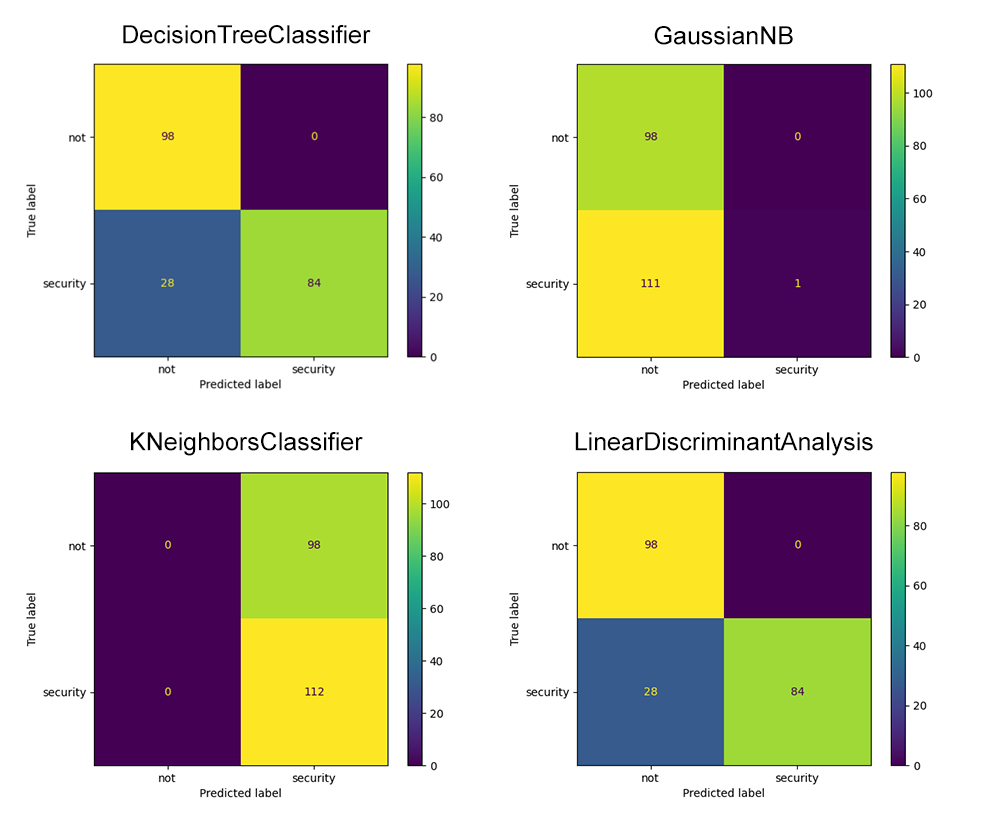
\includegraphics[width=25em]{../report/images/conf_mat_1.png}}
    \caption{Matrizes de Confusão 1}
    \label{fig:conf_mat_1}
  \end{figure}
\end{frame}

\begin{frame}
  \frametitle{Matrizes de Confusão}
  \begin{figure}[htbp]
    \centerline{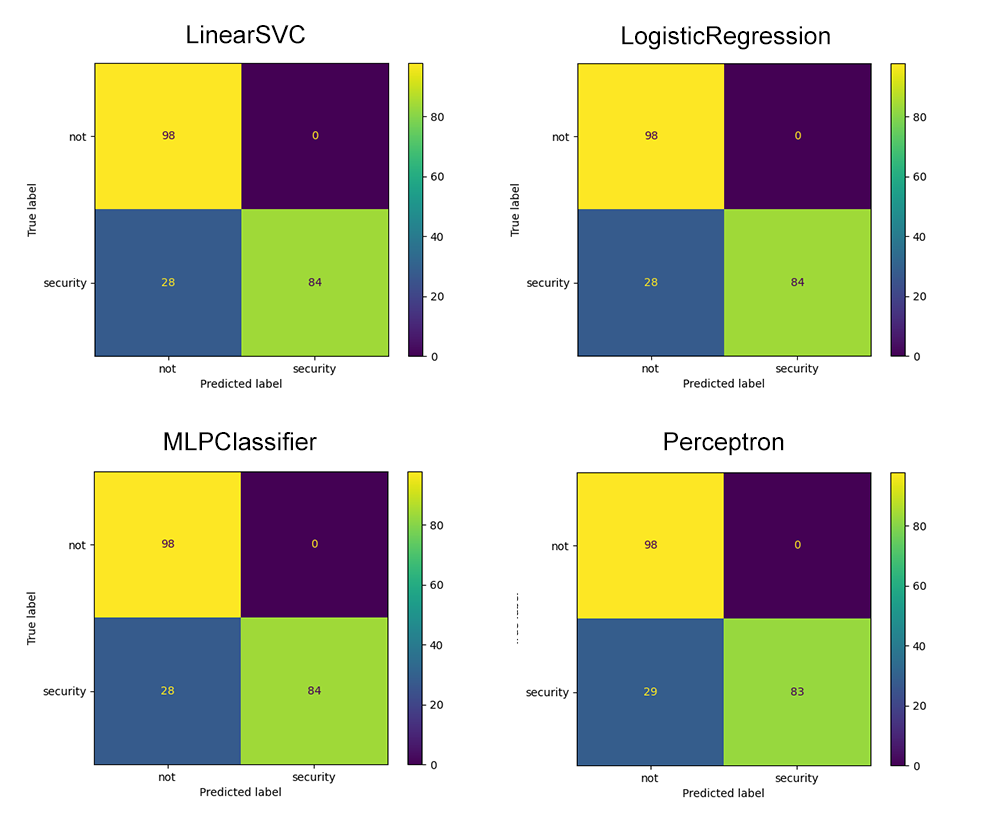
\includegraphics[width=25em]{../report/images/conf_mat_2.png}}
    \caption{Matrizes de Confusão 2}
    \label{fig:conf_mat_2}
  \end{figure}
\end{frame}